% NightShift: batch LLM inference on charging smartphones.
% Build:  latexmk -pdf main.tex          (anonymous review copy, default)
%         latexmk -pdf -jobname=main-arxiv -pdflatex='pdflatex %O "\def\arxiv{1}\input{%S}"' main.tex
\ifdefined\arxiv
  \documentclass[sigconf,nonacm]{acmart}
\else
  \documentclass[sigconf,review,anonymous]{acmart}
\fi
\settopmatter{printacmref=false}
\setcopyright{none}
\renewcommand\footnotetextcopyrightpermission[1]{}
\usepackage{booktabs}
% generated by sim/make_numbers.py; do not edit
\newcommand{\ActCA}{47}
\newcommand{\ActConsol}{44}
\newcommand{\ActLifetime}{50}
\newcommand{\ActNS}{26}
\newcommand{\ActNSNoWait}{46}
\newcommand{\ActReplay}{48}
\newcommand{\ActRestart}{0}
\newcommand{\ActStandby}{50}
\newcommand{\ActSticky}{48}
\newcommand{\ActWait}{51}
\newcommand{\CAvsReplayPct}{+2}
\newcommand{\CIConsCA}{1.7}
\newcommand{\CIConsConsol}{0.0}
\newcommand{\CIConsLifetime}{1.7}
\newcommand{\CIConsNS}{4.0}
\newcommand{\CIConsNSNoWait}{2.7}
\newcommand{\CIConsReplay}{1.7}
\newcommand{\CIConsRestart}{2.0}
\newcommand{\CIConsStandby}{2.5}
\newcommand{\CIConsSticky}{2.2}
\newcommand{\CIConsWait}{2.0}
\newcommand{\CIRepCA}{1.3}
\newcommand{\CIRepConsol}{1.7}
\newcommand{\CIRepLifetime}{1.4}
\newcommand{\CIRepNS}{5.1}
\newcommand{\CIRepNSNoWait}{4.0}
\newcommand{\CIRepReplay}{0.0}
\newcommand{\CIRepRestart}{0.4}
\newcommand{\CIRepStandby}{1.3}
\newcommand{\CIRepSticky}{2.8}
\newcommand{\CIRepWait}{3.5}
\newcommand{\CacheFullCA}{207}
\newcommand{\CacheFullConsol}{182}
\newcommand{\CacheFullNS}{40}
\newcommand{\CacheFullRatioCA}{5}
\newcommand{\CacheFullReplay}{213}
\newcommand{\CacheFullTputCA}{115}
\newcommand{\CacheFullTputConsol}{123}
\newcommand{\CacheFullTputNS}{109}
\newcommand{\CacheFullTputReplay}{114}
\newcommand{\ConsolGainPct}{+8}
\newcommand{\DiffConsCA}{-6.8}
\newcommand{\DiffConsConsol}{+0.0}
\newcommand{\DiffConsLifetime}{-13.2}
\newcommand{\DiffConsNS}{-6.0}
\newcommand{\DiffConsNSNoWait}{-14.8}
\newcommand{\DiffConsReplay}{-8.5}
\newcommand{\DiffConsRestart}{-12.2}
\newcommand{\DiffConsStandby}{-50.4}
\newcommand{\DiffConsSticky}{-20.0}
\newcommand{\DiffConsWait}{-21.6}
\newcommand{\DiffRepCA}{+1.7}
\newcommand{\DiffRepConsol}{+8.5}
\newcommand{\DiffRepLifetime}{-4.8}
\newcommand{\DiffRepNS}{+2.4}
\newcommand{\DiffRepNSNoWait}{-6.4}
\newcommand{\DiffRepReplay}{+0.0}
\newcommand{\DiffRepRestart}{-3.8}
\newcommand{\DiffRepStandby}{-41.9}
\newcommand{\DiffRepSticky}{-11.6}
\newcommand{\DiffRepWait}{-13.1}
\newcommand{\EligiblePct}{90}
\newcommand{\FailCA}{1490}
\newcommand{\FailConsol}{1452}
\newcommand{\FailDropPct}{46}
\newcommand{\FailLifetime}{1469}
\newcommand{\FailNS}{804}
\newcommand{\FailNSNoWait}{1257}
\newcommand{\FailReplay}{1487}
\newcommand{\FailRestart}{1487}
\newcommand{\FailStandby}{859}
\newcommand{\FailSticky}{1285}
\newcommand{\FailWait}{1314}
\newcommand{\GBCA}{363}
\newcommand{\GBConsol}{368}
\newcommand{\GBLifetime}{610}
\newcommand{\GBNS}{57}
\newcommand{\GBNSNoWait}{320}
\newcommand{\GBRatio}{7}
\newcommand{\GBRatioCA}{6}
\newcommand{\GBRatioConsol}{7}
\newcommand{\GBRatioMax}{12}
\newcommand{\GBRatioMin}{2}
\newcommand{\GBReplay}{410}
\newcommand{\GBRestart}{375}
\newcommand{\GBStandby}{492}
\newcommand{\GBSticky}{296}
\newcommand{\GBWait}{302}
\newcommand{\JCA}{7}
\newcommand{\JConsol}{6}
\newcommand{\JLifetime}{7}
\newcommand{\JNS}{6}
\newcommand{\JNSNoWait}{6}
\newcommand{\JReplay}{7}
\newcommand{\JRestart}{7}
\newcommand{\JStandby}{6}
\newcommand{\JSticky}{7}
\newcommand{\JWait}{7}
\newcommand{\LatCA}{2.3}
\newcommand{\LatConsol}{2.3}
\newcommand{\LatLAN}{2.0}
\newcommand{\LatLifetime}{2.3}
\newcommand{\LatNS}{2.3}
\newcommand{\LatNSNoWait}{2.3}
\newcommand{\LatReplay}{2.3}
\newcommand{\LatRestart}{2.3}
\newcommand{\LatSlow}{3.2}
\newcommand{\LatStandby}{2.3}
\newcommand{\LatSticky}{2.3}
\newcommand{\LatWAN}{2.3}
\newcommand{\LatWait}{2.3}
\newcommand{\MinAvail}{35}
\newcommand{\NPhones}{1{,}000}
\newcommand{\NSbehindConsolPct}{5}
\newcommand{\NSvsCAPct}{+1}
\newcommand{\NSvsConsolPct}{-5}
\newcommand{\NSvsReplayPct}{+2}
\newcommand{\NightSharePct}{98}
\newcommand{\OracleCA}{66}
\newcommand{\OracleConsol}{70}
\newcommand{\OracleLifetime}{62}
\newcommand{\OracleNS}{66}
\newcommand{\OracleNSNoWait}{61}
\newcommand{\OracleReplay}{65}
\newcommand{\OracleRestart}{71}
\newcommand{\OracleStandby}{39}
\newcommand{\OracleSticky}{58}
\newcommand{\OracleWait}{57}
\newcommand{\PeakAvail}{731}
\newcommand{\PeakPipes}{36}
\newcommand{\PhoneGBCA}{4.0}
\newcommand{\PhoneGBConsol}{4.3}
\newcommand{\PhoneGBLifetime}{6.3}
\newcommand{\PhoneGBNS}{0.7}
\newcommand{\PhoneGBNSNoWait}{3.4}
\newcommand{\PhoneGBReplay}{4.4}
\newcommand{\PhoneGBRestart}{3.9}
\newcommand{\PhoneGBStandby}{3.2}
\newcommand{\PhoneGBSticky}{3.0}
\newcommand{\PhoneGBWait}{2.9}
\newcommand{\PoolLargeGBNS}{35}
\newcommand{\PoolLargeGBRatio}{12}
\newcommand{\PoolLargeGBRatioCA}{10}
\newcommand{\PoolLargeGBReplay}{428}
\newcommand{\PoolLargeGainPct}{+17}
\newcommand{\PoolLargeVsConsolPct}{+7}
\newcommand{\PoolSmallGBNS}{162}
\newcommand{\PoolSmallGBRatio}{2}
\newcommand{\PoolSmallGBRatioCA}{2}
\newcommand{\PoolSmallGBReplay}{374}
\newcommand{\PoolSmallGainPct}{-9}
\newcommand{\PoolSmallVsConsolPct}{-14}
\newcommand{\RestartVsReplayPct}{-4}
\newcommand{\Seeds}{5}
\newcommand{\ShardCA}{316}
\newcommand{\ShardConsol}{323}
\newcommand{\ShardLifetime}{561}
\newcommand{\ShardNS}{30}
\newcommand{\ShardNSNoWait}{273}
\newcommand{\ShardRatio}{12}
\newcommand{\ShardReplay}{362}
\newcommand{\ShardRestart}{375}
\newcommand{\ShardStandby}{443}
\newcommand{\ShardSticky}{247}
\newcommand{\ShardWait}{251}
\newcommand{\StandbyDropPct}{39}
\newcommand{\StickyGainPct}{-11}
\newcommand{\SwBatchHiNS}{146}
\newcommand{\SwBatchHiReplay}{145}
\newcommand{\SwBatchLoNS}{61}
\newcommand{\SwBatchLoReplay}{59}
\newcommand{\SwDayDurHiNS}{121}
\newcommand{\SwDayDurHiReplay}{119}
\newcommand{\SwDayDurLoNS}{105}
\newcommand{\SwDayDurLoReplay}{109}
\newcommand{\SwHopHiNS}{76}
\newcommand{\SwHopHiReplay}{75}
\newcommand{\SwHopLoNS}{120}
\newcommand{\SwHopLoReplay}{119}
\newcommand{\SwNightHiNS}{138}
\newcommand{\SwNightHiReplay}{129}
\newcommand{\SwNightLoNS}{58}
\newcommand{\SwNightLoReplay}{63}
\newcommand{\SwPoolHiCA}{110}
\newcommand{\SwPoolHiConsol}{119}
\newcommand{\SwPoolHiNS}{127}
\newcommand{\SwPoolHiReplay}{109}
\newcommand{\SwPoolLoCA}{109}
\newcommand{\SwPoolLoConsol}{115}
\newcommand{\SwPoolLoNS}{98}
\newcommand{\SwPoolLoReplay}{108}
\newcommand{\SwPrefillHiNS}{134}
\newcommand{\SwPrefillHiReplay}{132}
\newcommand{\SwPrefillLoNS}{58}
\newcommand{\SwPrefillLoReplay}{59}
\newcommand{\TputCA}{108}
\newcommand{\TputConsol}{115}
\newcommand{\TputGainPct}{2}
\newcommand{\TputLifetime}{101}
\newcommand{\TputNS}{109}
\newcommand{\TputNSNoWait}{100}
\newcommand{\TputReplay}{106}
\newcommand{\TputRestart}{102}
\newcommand{\TputSDCA}{2.4}
\newcommand{\TputSDConsol}{2.9}
\newcommand{\TputSDLifetime}{2.4}
\newcommand{\TputSDNS}{4.9}
\newcommand{\TputSDNSNoWait}{4.1}
\newcommand{\TputSDReplay}{1.7}
\newcommand{\TputSDRestart}{1.5}
\newcommand{\TputSDStandby}{1.5}
\newcommand{\TputSDSticky}{3.3}
\newcommand{\TputSDWait}{4.1}
\newcommand{\TputStandby}{64}
\newcommand{\TputSticky}{95}
\newcommand{\TputWait}{93}
\newcommand{\UsefulCA}{65}
\newcommand{\UsefulConsol}{70}
\newcommand{\UsefulLifetime}{61}
\newcommand{\UsefulNS}{83}
\newcommand{\UsefulNSNoWait}{69}
\newcommand{\UsefulReplay}{64}
\newcommand{\UsefulRestart}{70}
\newcommand{\UsefulStandby}{74}
\newcommand{\UsefulSticky}{65}
\newcommand{\UsefulWait}{64}
\newcommand{\WaitSixtyGB}{109}
\newcommand{\WaitSixtyTput}{107}
\newcommand{\WaitTenGB}{45}
\newcommand{\WaitTenTput}{108}
\newcommand{\WaitZeroGB}{314}
\newcommand{\WaitZeroTput}{99}
\newcommand{\WaitvsCAPct}{-14}


% Placeholders that only real measurements can fill are printed in this colour
% and listed in the handoff. A submission must contain none of them.
\newcommand{\TODO}[1]{\textcolor{red}{[#1]}}

\begin{document}

\title{NightShift: Batch LLM Inference on Charging Smartphones}

\author{Aidin Bazarchi}
\affiliation{%
  \institution{Independent Researcher}
  \country{}}

\begin{abstract}
Many smartphones spend the night plugged in, on Wi-Fi and idle.
We ask whether such a pool can run inference for a large language model too
big for any single phone, and what it would take. A 70B-parameter model at
4-bit needs about 40\,GB, so one copy is a 16-stage pipeline of phones that
leave whenever their owners unplug them. Using a simulator whose phone and
network parameters are explicit, replaceable assumptions, we find three
things. First, the pool is a night-time resource: \NightSharePct\% of a day's
tokens are produced between 22:00 and 08:00. Second, each output token takes
seconds (\LatWAN\,s at 60\,ms per hop), so the useful workload is batch work,
not chat. Third, once phones come and go, the main cost of churn is moving
model shards to the phones that replace leavers, not recomputing lost work:
even a cache-aware baseline downloads \GBCA\,GB per million tokens, about
\PhoneGBCA\,GB per serving phone per day. NightShift gives every phone a
permanent home block, lets a vacant stage wait briefly for a phone that
already holds it, and consolidates broken pipelines. With 1,000 phones it
downloads \GBRatioCA--\GBRatio$\times$ less data than every baseline we
compare, with throughput equal to Petals-style replay within noise and
\NSbehindConsolPct\% below the best baseline; at 4,000 phones it is ahead on both
(\PoolLargeVsConsolPct\% throughput against consolidation, \PoolLargeGBRatioCA$\times$ less traffic than cache-aware).
Keeping warm standbys, the obvious remedy, cuts throughput by
\StandbyDropPct\%. We release the simulator and a benchmark kit so that the
assumed parameters can be replaced with measurements.
\end{abstract}

\begin{CCSXML}
<ccs2012>
<concept><concept_id>10010520.10010521.10010537</concept_id>
<concept_desc>Computer systems organization~Distributed architectures</concept_desc>
<concept_significance>500</concept_significance></concept>
<concept><concept_id>10003120.10003138</concept_id>
<concept_desc>Human-centered computing~Ubiquitous and mobile computing</concept_desc>
<concept_significance>300</concept_significance></concept>
<concept><concept_id>10010147.10010257</concept_id>
<concept_desc>Computing methodologies~Machine learning</concept_desc>
<concept_significance>300</concept_significance></concept>
</ccs2012>
\end{CCSXML}
\ccsdesc[500]{Computer systems organization~Distributed architectures}
\ccsdesc[300]{Human-centered computing~Ubiquitous and mobile computing}
\ccsdesc[300]{Computing methodologies~Machine learning}
\keywords{large language models, distributed inference, smartphones, volunteer computing, pipeline parallelism, churn}

\maketitle

\section{Introduction}

Volunteer computing has a long record: BOINC and SETI@home turned idle desktops
into a scientific computer~\cite{boinc}, and Google's federated learning system
trains models on phones only while they are ``idle, charging and on an
unmetered network''~\cite{bonawitz2019}. Large language models (LLMs) are the
largest compute consumer of the decade, which invites the question: could the
idle phones of the world run them?

The question has an easy wrong answer in each direction. ``Yes, a billion
phones beat any data centre'' ignores that generation is sequential and that a
large model does not fit on a phone. ``No, phones are too small'' ignores that
the same was said of volunteer desktops, and that systems such as
Petals~\cite{petals-acl,petals-neurips} already serve 100B-class models from
pipelines of volunteer GPUs over the internet. The interesting question is
quantitative: \emph{for which workloads, at what throughput and cost, and
which design choices matter?}

This paper makes three contributions.
\begin{enumerate}
\item A first-principles analysis (\S\ref{sec:physics}) of what a phone pool
can and cannot do: it suits throughput-oriented batch jobs, not interactive
chat, and it reads far more weight memory per token than a GPU, so its case rests on marginal cost, not efficiency.
\item A churn-aware simulator (\S\ref{sec:method}) driven by a diurnal model of
when phones are charging and on Wi-Fi. Every phone, network and user parameter
is explicit and can be replaced by a measurement; we release a benchmark kit
that produces those measurements on Android phones.
\item NightShift (\S\ref{sec:design}), a placement and recovery design built on
one observation from the simulator: once phones come and go, moving model
shards costs more than redoing computation. A permanent home block per phone,
a short wait for a phone that holds the vacant block, and consolidation of
broken pipelines cut data downloaded \GBRatioCA--\GBRatio$\times$ against
every baseline at 1,000 phones, including a fair cache-aware one, and
\CacheFullRatioCA$\times$ even when phones cache the whole model. Throughput matches replay within noise and is
\NSbehindConsolPct\% below the best baseline at this size; NightShift's lead
grows with the pool, and it trails at 500 phones. An ablation shows that
neither the wait nor consolidation helps alone, and that dedicated standbys
make things worse.
\end{enumerate}

We are explicit about what is and is not measured. All results here come from
simulation with stated assumptions (Table~\ref{tab:params}); \S\ref{sec:validation}
describes the measurements that will replace them.

\section{The physics of a phone pool}
\label{sec:physics}

\paragraph{Memory.} A 70B model quantised to about 4 bits per weight occupies
roughly 40\,GB; we model 80 layers of 0.5\,GB. An Android app running in the
background can rarely hold more than a fraction of a phone's RAM; we assume
45\%, so an 8\,GB phone offers 3.6\,GB. With the key-value (KV) cache for a
batch of 32 sequences of 768 tokens, a five-layer block needs 3.0\,GB, so a
model copy is a pipeline of 16 phones, and phones with 6\,GB of RAM cannot take
part at all (\EligiblePct\% of our pool is eligible).

\paragraph{Latency.} Generating one token visits all 16 stages in order. At
roughly 15\,ms per layer on a mid-range phone and 60\,ms per wide-area hop,
a token takes about 1.2\,s of compute plus 1.0\,s of network, i.e.\ around two
seconds. Neither speculative decoding~\cite{specdec} nor faster phones change
the order of magnitude while the hops remain. A conversational assistant is
therefore out of reach over the internet; a household network
(5\,ms hops) brings latency to \LatLAN\,s.

\paragraph{Throughput.} Latency need not limit throughput. With many sequences
in flight, a pipeline keeps every stage busy, as in GPipe-style
micro-batching~\cite{gpipe} and continuous batching servers~\cite{orca,vllm}.
Batch workloads such as offline evaluation, synthetic data generation,
document summarisation or embedding a corpus tolerate hours of latency and are
a large share of LLM demand, the same regime FlexGen targets on a single
GPU~\cite{flexgen}.

\paragraph{Memory traffic and energy.} The price is efficiency. A data-centre
GPU serving a batch of 128 reads each weight once per 128 tokens, about
0.3\,GB of weight traffic per token for a 70B model. A phone pipeline with 32
sequences over 16 stages processes micro-batches of two, so it reads about
20\,GB per token, roughly 60$\times$ more. At an assumed 4\,W per active phone and
1\,W while waiting, the simulated pool spends about \JNS\,J per token; we have
not measured a GPU server on the same workload, and that comparison is part of
the validation plan. The phone pool's argument is therefore not
efficiency but \emph{marginal cost}: the hardware is already bought, already
powered at night and otherwise idle. Whether that argument survives battery
wear and the owner's electricity bill is a question for measurement and
incentive design, which we leave open (\S\ref{sec:limits}).

\section{Related work}

\paragraph{Volunteer and federated computing.} BOINC~\cite{boinc} established
redundant execution and work units for untrusted volunteers but ran independent
jobs. Federated learning~\cite{fedavg,bonawitz2019} runs on phones at
production scale and established the eligibility rule we adopt (charging,
Wi-Fi, idle); each phone trains a full small model, and nothing is split across
devices. Device availability in federated learning has been measured at large
scale~\cite{yang2021heterogeneity,fedscale}; those traces are natural inputs
to our simulator.

\paragraph{LLMs over unreliable consumer hardware.}
Petals~\cite{petals-acl,petals-neurips} serves large models from pipelines of
volunteer GPUs and recovers from departures by routing around them and
replaying the lost stage's cache; it is the baseline we call \emph{replay}.
SWARM~\cite{swarm}, Learn\-ing\-@home~\cite{learningathome} and
DiLoCo~\cite{diloco} train over unreliable or poorly connected nodes.
Deserve~\cite{deserve} studies decentralised serving on volunteer GPUs, and
HexGen~\cite{hexgen} schedules LLM inference over heterogeneous, decentralised
GPUs. SpotServe~\cite{spotserve} serves LLMs on preemptible cloud instances,
migrating context when an instance is reclaimed. For training,
Bamboo~\cite{bamboo} adds redundant computation and Oobleck~\cite{oobleck}
keeps redundant pipeline templates to survive failures, and
Parcae~\cite{parcae} predicts spot-instance availability to adapt
parallelism proactively, the same idea as our lifetime grouping. Those nodes
are GPUs with tens of gigabytes and, often, minutes of warning; ours are phones
with a few gigabytes and no warning, and moving a shard to a replacement costs
the volunteer data.

\paragraph{Splitting models across nearby devices.}
LinguaLinked~\cite{lingualinked} runs one LLM across several Android phones,
Galaxy~\cite{galaxy} and EdgeShard~\cite{edgeshard} split transformers across
edge devices, and exo~\cite{exo} does so for a household's laptops and phones;
prima.cpp~\cite{primacpp} runs 70B-class models on a home cluster of
everyday devices; earlier, MoDNN~\cite{modnn} and DeepThings~\cite{deepthings}
split CNNs, and CWC~\cite{cwc} scheduled jobs on the idle, charging phones of
an organisation. These
assume a small, stable set of devices. We study the opposite regime: a large
pool in which membership changes all the time.

\paragraph{Single-phone inference.} LLM in a flash~\cite{llminaflash},
PowerInfer-2~\cite{powerinfer2} and runtimes such as llama.cpp~\cite{llamacpp}
make single phones faster, and MobileLLM~\cite{mobilellm} designs models that
fit one phone. These are complementary: a faster phone shortens every stage,
and a model that fits one phone needs no pipeline at all, which is the right
choice whenever such a model is good enough.

\section{NightShift}
\label{sec:design}

A coordinator holds a job queue and a fixed \emph{shard catalogue}: the model
cut into 16 blocks of 5 layers. A phone joins the pool when it is charging, on
Wi-Fi and idle, and leaves without warning. A pipeline is one phone per block;
it advances a batch of 32 sequences in lock step. When a member leaves, its
sequences pause until the stage is refilled. NightShift has three parts.

\paragraph{Sticky shards.} Every phone is assigned a \emph{home block} once
and keeps it in flash storage indefinitely. A pipeline stage is only ever
filled by a phone whose home block matches; loading from flash takes seconds,
whereas downloading 2.5\,GB over a residential link takes minutes and costs the
owner data. If no matching phone is idle, the vacant stage waits up to five
minutes before falling back to a phone that must download the block; a
pipeline whose stage has been vacant for ten minutes is dissolved and its
phones return to the pool (this rule applies to every policy).
Because the catalogue is fixed, the coordinator only needs to keep the 16
home-block populations balanced.

\paragraph{Lifetime-grouped pipelines.} A pipeline lives only as long as its
shortest-lived member. The coordinator predicts when each phone's charging
session ends, from that user's history of sessions starting at a similar time
of day, sorts each block's idle phones by predicted end, and builds the $i$-th
pipeline from the $i$-th phone of every block. Phones expected to stay until
morning end up together, and short daytime sessions are grouped with each
other instead of cutting long-lived pipelines short.

\paragraph{Dawn consolidation.} In the morning, phones leave faster than idle
phones arrive, leaving many pipelines with one or two vacant stages that
nobody can fill. Waiting wastes every phone in those pipelines. When at least
two pipelines are broken, NightShift dissolves the most damaged one (most
vacancies, then least progress) and lends its phones, which already hold blocks
of the same catalogue, to the others. A pool that shrinks keeps as many
\emph{complete} pipelines as it can afford. Because the donor's phones hold the
blocks the survivors are missing, consolidation is also what keeps the wait
short: without it, a vacant stage often waits for a home-block phone that is
not coming.

\paragraph{Recovery.} A replacement phone recomputes the KV cache of its block
for the tokens processed so far, as in Petals. To do so it needs the input
activations of its block for every token so far (prompt and generated). We
assume the previous stage keeps them and sends them over the replacement's
downlink, 16\,KiB per token per sequence (8,192 hidden dimensions in fp16);
this transfer takes time and is counted as traffic for every policy. We
compare replay with restarting the batch.

\paragraph{What we chose not to do.} Keeping $k$ warm standbys per stage turns a
failure into a fast swap but takes $k\times16$ phones out of service per
pipeline. We evaluate it as a baseline.

\section{Simulation methodology}
\label{sec:method}

\begin{table}[t]
\caption{Simulator parameters. All are assumptions until replaced by
measurements from the benchmark kit (\S\ref{sec:validation}).}
\label{tab:params}
\small
\begin{tabular}{@{}p{0.25\columnwidth}p{0.71\columnwidth}@{}}
\toprule
Model & 80 layers $\times$ 0.5\,GB, KV 4\,KiB/token/layer\\
Workload & batches of 32 seq., 512 prompt + 256 output tokens\\
Prefill cost & 1/8 of a decode token\\
Phones & RAM, share of pool, ms per layer: 6\,GB, 10\%, 30; 8\,GB, 40\%, 18; 12\,GB, 35\%, 12; 16\,GB, 15\%, 10 (log-normal spread $\sigma{=}0.2$)\\
Usable RAM & 45\% of physical\\
Network & 60\,ms per hop; downlink median 50\,Mbit/s\\
Flash read & 1\,GB/s\\
Power & 4\,W computing, 1\,W waiting\\
Night charging & 85\% of nights, start 23:00$\pm$1\,h, 7$\pm$1.5\,h\\
Day charging & 1.5 sessions/day, median 35\,min, 60\% on Wi-Fi\\
Flash cache & 1 block (2.5\,GB) per phone; \S\ref{sec:results} varies it to 16\\
Activations & 16\,KiB per token per sequence, sent on repair\\
Timers & home-block wait 300\,s; vacant pipeline dissolved after 600\,s\\
Warm-up & 2 days run and discarded before measuring\\
\bottomrule
\end{tabular}
\end{table}

The simulator advances in 10-second ticks. Each phone has a RAM class, a
per-layer decode time and a downlink speed drawn from Table~\ref{tab:params},
and a sequence of charging sessions drawn from the diurnal model, or read from
a real trace. A pipeline's \emph{time per output token} is one round: the sum
of its stage times plus one hop per stage. With 16 micro-batches in flight, a
round is $\max(\text{latency}, 16\cdot\max_i \text{stage}_i)$ and produces one
token for each of the 32 sequences. A micro-batch of $b$ tokens costs
$1+0.1(b-1)$ times a single token, and prefill costs 1/8 of a decode token.

\paragraph{Steady state.} Seven days of synthetic history train the session-end
predictor. The simulator then runs two days under the policy being evaluated
and discards them, so that flash caches and pipelines reach that policy's own
steady state, and finally measures 24 hours from noon. Every phone starts the
warm-up holding one block (its home block), so a policy cannot look good merely
by inheriting another's caches. Onboarding traffic, a phone's first download,
is outside the measured window for every policy.

\paragraph{Policies.} We compare ten policies that differ only in placement and
recovery. The baselines are \emph{restart} and \emph{replay} (random placement;
restart a broken batch, or replay its cache as Petals does);
\emph{cache-aware}, a fair version of replay that fills each stage from idle
phones already holding its block before falling back to any idle phone (it
never waits); \emph{standby} (replay plus one warm standby per stage);
\emph{lifetime} (replay with pipelines grouped by predicted session end); and
\emph{consolidate} (replay plus consolidation). The NightShift ablation adds
one part at a time: \emph{wait} (home blocks and the five-minute wait, random
order), \emph{sticky} (plus lifetime grouping), \emph{NightShift without the
wait} (sticky plus consolidation, falling back to a download at once) and
\emph{NightShift}. The \emph{upper bound} places every available, eligible
phone in a complete pipeline instantly and never loses work.

\paragraph{Metrics and statistics.} Throughput is output tokens per second per
1,000 phones in the pool. Traffic is gigabytes downloaded per million output
tokens: shards plus repair activations. Results are means over \Seeds{} seeds
with \NPhones{} phones (sweeps: 3 seeds); differences between policies are
paired by seed, so both see the same phones and sessions, and we report them
with 95\% $t$ confidence intervals.

\section{Results}
\label{sec:results}

\begin{figure}[t]
\centering
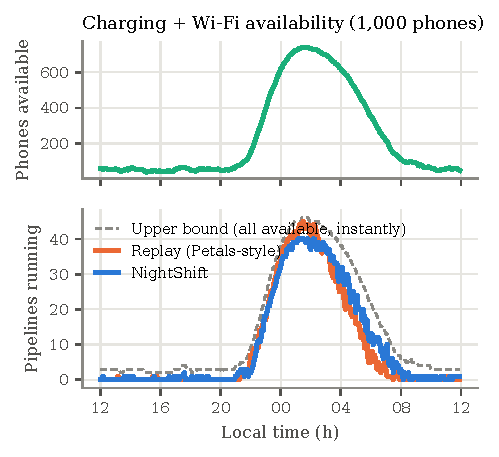
\includegraphics[width=\columnwidth]{figures/timeline}
\Description{Two stacked line charts over 24 hours. Top: number of available phones, low during the day and peaking at night. Bottom: running pipelines for replay and NightShift against an upper bound; nearly all pipelines run between 22:00 and 08:00.}
\caption{One simulated day. Top: phones available. Bottom: pipelines running
and an upper bound that assumes instant, perfect placement.}
\label{fig:timeline}
\end{figure}

\paragraph{The pool is a night-time machine.} Availability swings from
\MinAvail{} to \PeakAvail{} of 1,000 phones over the day
(Figure~\ref{fig:timeline}), and \NightSharePct\% of tokens are produced
between 22:00 and 08:00. Daytime sessions are short and scattered, so few
complete 16-phone pipelines form. A phone pool is best treated as a batch
system that drains a queue overnight.

\begin{figure*}[t]
\centering
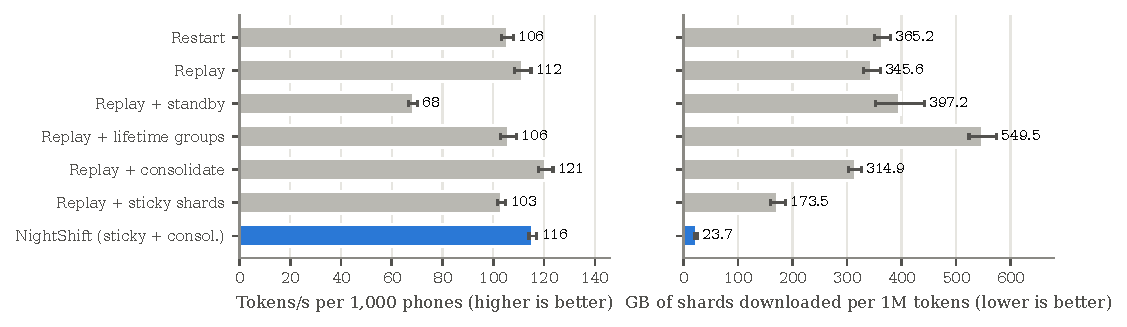
\includegraphics[width=\textwidth]{figures/policies}
\Description{Two horizontal bar charts comparing ten policies. Left: tokens per second per 1,000 phones, between 64 (replay with standby) and 115 (replay with consolidation); NightShift is 109. Right: gigabytes downloaded per million tokens, split into shards and activations; the baselines range from 296 to 610 and NightShift is 57.}
\caption{Throughput and data downloaded (shards, dark; repair activations,
light) of the ten policies (1,000 phones, mean $\pm$ s.d.\ over \Seeds{}
seeds). The last four rows add NightShift's parts one at a time.}
\label{fig:policies}
\end{figure*}

\paragraph{Moving shards, not lost work, is the cost of churn.}
Figure~\ref{fig:policies} compares the policies. Restart differs from replay by only
\RestartVsReplayPct\% ($\pm$\CIRepRestart{} tokens/s, 95\% CI),
so little computation is lost to departures. What separates the policies is
data movement. Under replay, a repair recruits whichever phone is idle, which
rarely holds the needed block: the pool downloads \GBReplay\,GB per million
tokens, of which \ShardReplay\,GB are shards. Preferring phones that already
hold the block (cache-aware) helps less than one would expect, to \GBCA\,GB,
because at a given moment the few idle phones seldom hold the right block; a
serving phone still downloads about \PhoneGBCA\,GB a day, enough to make a
volunteer's data plan the binding constraint.

\paragraph{NightShift.} NightShift downloads \GBNS\,GB per million tokens:
\GBRatio$\times$ less than replay, \GBRatioCA$\times$ less than cache-aware and
\GBRatioConsol$\times$ less than consolidation; for shards alone the reduction
against replay is \ShardRatio$\times$. A serving phone downloads about
\PhoneGBNS\,GB a day instead of \PhoneGBReplay\,GB. Its throughput is
\TputNS{} tokens/s per 1,000 phones against \TputReplay{} for replay, a paired
difference of \DiffRepNS{} $\pm$ \CIRepNS, which is not significant. The best
baseline, consolidation, is faster: \TputConsol{} tokens/s, a paired difference of
\DiffConsNS{} $\pm$ \CIConsNS{} tokens/s, so NightShift is
\NSbehindConsolPct\% behind it at this pool size. NightShift suffers \FailDropPct\% fewer stage failures than replay,
and its stages spend \UsefulNS\% of their time computing rather than waiting,
against \UsefulReplay\%. The trade is therefore a few percent of throughput
at 1,000 phones for a large cut in the data volunteers must download.

\paragraph{The ablation: the wait and consolidation need each other.}
Giving each phone a home block and making vacant stages wait for it
(\emph{wait}) cuts traffic only to \GBWait\,GB and changes throughput by
\DiffRepWait{} $\pm$ \CIRepWait{} tokens/s against replay: in the morning,
stages wait for home-block phones that have left for the day. Adding lifetime
grouping changes little (\TputSticky{} tokens/s, \GBSticky\,GB). Adding
consolidation but no wait (\emph{NightShift without the wait}) recovers some
throughput but keeps traffic at \GBNSNoWait\,GB, because every vacancy still
triggers a download. Only together does the design work: consolidation
supplies home-block phones from dissolved pipelines, so the wait is usually
short and usually rewarded. Lifetime grouping alone, without home blocks, is
worse than random (\TputLifetime{} tokens/s, \GBLifetime\,GB), because ranking
phones by predicted stay overrides any chance of reusing a cached block.

\paragraph{Standbys are a bad trade on phones.} One standby per stage cuts
throughput by \StandbyDropPct\%: it removes half of the pool from service to
protect pipelines whose expected lifetime, at night, is hours. Redundancy pays
off when failures are frequent relative to the cost of idling capacity, as for
preemptible cloud GPUs~\cite{bamboo,oobleck}, but not here.

\begin{figure}[t]
\centering
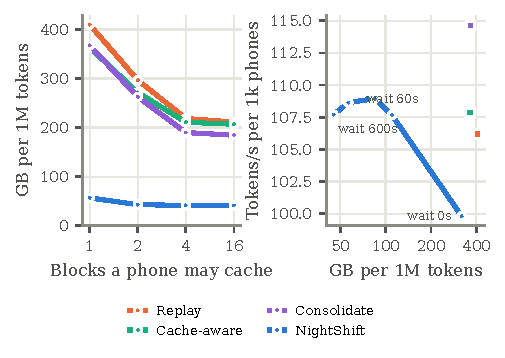
\includegraphics[width=\columnwidth]{figures/tradeoff}
\Description{Left: line chart of gigabytes downloaded per million tokens against the number of blocks a phone may cache (1, 2, 4, 16). Replay, cache-aware and consolidate fall from about 400 to about 200; NightShift stays near 40 to 55. Right: throughput against traffic on a log axis. NightShift's points for waits of 0 to 600 seconds trace a curve from about 99 tokens per second at 314 GB to about 108 at 45 GB; square markers show replay, cache-aware and consolidate at 360 to 410 GB.}
\caption{Left: traffic when each phone may cache more blocks. Right: throughput
against traffic; NightShift's wait time (0--600\,s) traces a trade-off, squares
are baselines.}
\label{fig:tradeoff}
\end{figure}

\paragraph{Larger caches do not close the gap.} One might expect the baselines
to catch up if phones simply kept more blocks in flash. Figure~\ref{fig:tradeoff}
(left) varies the cache from one block to all 16 (the whole 40\,GB model).
Baseline traffic roughly halves (replay \CacheFullReplay, cache-aware
\CacheFullCA, consolidation \CacheFullConsol\,GB per million tokens with a
full cache) while NightShift falls to \CacheFullNS\,GB, still
\CacheFullRatioCA$\times$ less than cache-aware. Keeping 40\,GB on a
volunteer's phone is, in any case, a large request; we assume one block.

\paragraph{The wait is a knob.} Figure~\ref{fig:tradeoff} (right) varies how
long a vacant stage waits for a home-block phone. With no wait, NightShift is
the no-wait ablation above (\WaitZeroTput{} tokens/s, \WaitZeroGB\,GB). A
60-second wait already gives \WaitSixtyTput{} tokens/s at \WaitSixtyGB\,GB,
and 600\,s gives \WaitTenTput{} tokens/s at \WaitTenGB\,GB. Throughput is
nearly flat beyond a minute while traffic keeps falling, so an operator can
choose the point that suits the volunteers' data plans.

\begin{figure}[t]
\centering
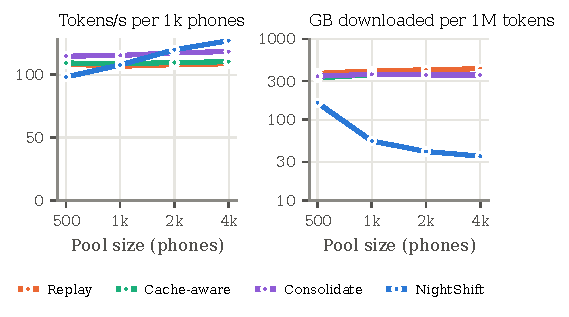
\includegraphics[width=\columnwidth]{figures/scale}
\Description{Two line charts against pool size from 500 to 4,000 phones for replay, cache-aware, consolidate and NightShift. Left: the three baselines stay flat between about 108 and 119 tokens per second per 1,000 phones, while NightShift rises from about 98 to 127, crossing consolidate near 2,000 phones. Right, log scale: the baselines stay between about 330 and 430 GB per million tokens while NightShift falls from about 160 to 35.}
\caption{NightShift improves with pool size; the baselines do not. Traffic
(shards plus activations) is on a logarithmic scale.}
\label{fig:scale}
\end{figure}

\paragraph{NightShift gets better with scale.} With more phones, each block
has more idle owners to choose from, so a vacant stage rarely waits long or
falls back to a download (Figure~\ref{fig:scale}). From 500 to 4,000 phones,
NightShift's throughput rises from \SwPoolLoNS{} to \SwPoolHiNS{} tokens/s per
1,000 phones and its traffic falls from \PoolSmallGBNS{} to
\PoolLargeGBNS\,GB per million tokens, while the baselines stay roughly flat
(replay \SwPoolLoReplay{} to \SwPoolHiReplay, consolidation
\SwPoolLoConsol{} to \SwPoolHiConsol). At 500 phones NightShift is worse:
\PoolSmallGainPct\% against replay and \PoolSmallVsConsolPct\% against
consolidation, with only \PoolSmallGBRatio$\times$ less traffic. At 4,000 it is
\PoolLargeGainPct\% against replay and \PoolLargeVsConsolPct\% against
consolidation, with \PoolLargeGBRatio$\times$ less traffic than replay. A
deployment worth building would have far more than 4,000 phones, but we have
not simulated beyond that, and a large pool would likely be split by region
(below), which brings each region back toward smaller pools.

\begin{figure*}[t]
\centering
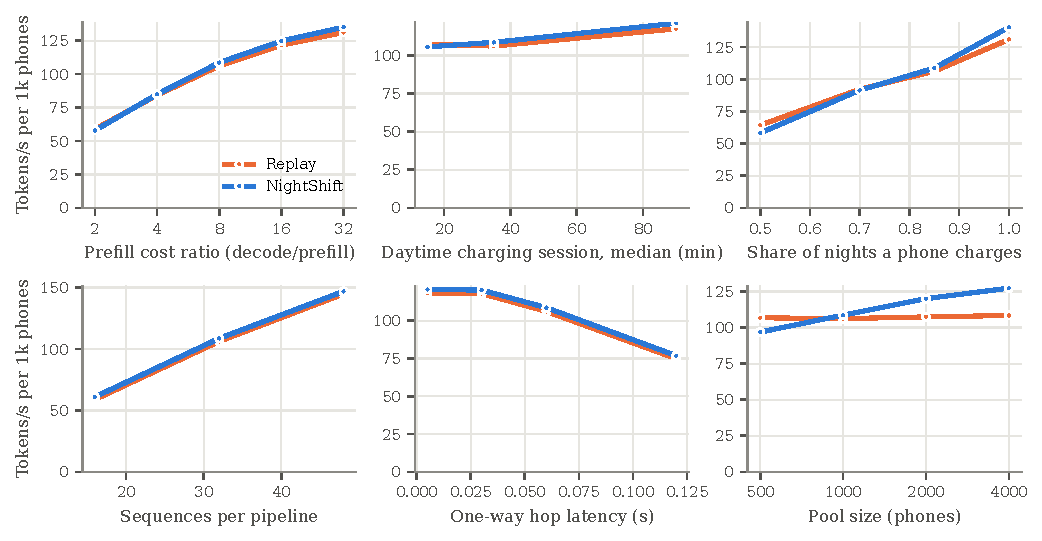
\includegraphics[width=\textwidth]{figures/sweeps}
\Description{Six small line charts of throughput for replay and NightShift as one assumption varies: prefill cost ratio, daytime session length, share of phones charging at night, sequences per pipeline, hop latency and pool size. The two policies track each other closely in most panels; NightShift pulls ahead at large pools and when most phones charge every night.}
\caption{Sensitivity of throughput to the main assumptions, replay vs.\
NightShift (1,000 phones, mean of 3 seeds).}
\label{fig:sweeps}
\end{figure*}

\paragraph{Sensitivity.} Figure~\ref{fig:sweeps} varies one assumption at a
time. Three matter a lot. The share of nights a phone charges moves
NightShift's throughput from \SwNightLoNS{} to \SwNightHiNS{} tokens/s per
1,000 phones between 50\% and 100\% of nights (at 50\%, replay is slightly
ahead). The batch size moves it from \SwBatchLoNS{} (16 sequences) to
\SwBatchHiNS{} (48), because more sequences keep more stages busy; memory for
the KV cache caps this. The cost ratio of decode to prefill moves it from
\SwPrefillLoNS{} (ratio 2) to \SwPrefillHiNS{} (ratio 32): the prompt of every
batch is processed once per stage, and each repair recomputes the cache of all
tokens so far.
Longer daytime sessions help only modestly (\SwDayDurLoNS{} to
\SwDayDurHiNS), confirming that the night carries the system. Hop latency
sets per-token latency (Figure~\ref{fig:latency}: \LatLAN\,s at 5\,ms,
\LatWAN\,s at 60\,ms, \LatSlow\,s at 120\,ms) and, because a round cannot be
shorter than one token's trip, also throughput (\SwHopLoNS{} to \SwHopHiNS).
Grouping pipelines by region, so that hops stay short, is therefore worth more
than any scheduling refinement. Across every setting we tried, NightShift
downloads \GBRatioMin--\GBRatioMax$\times$ less than replay, the low end at
500 phones; its throughput stays within a few percent of replay's except at
500 phones and at 50\% of nights, where it is behind.

\begin{figure}[t]
\centering
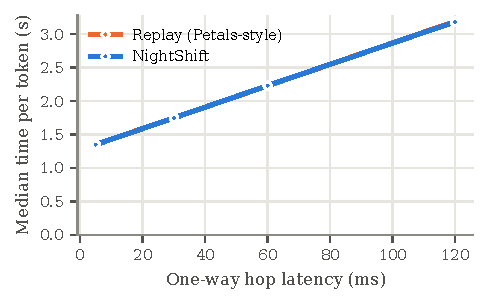
\includegraphics[width=0.92\columnwidth]{figures/latency}
\Description{Line chart of median time per output token against one-way hop latency from 5 to 120 ms; it rises from about 2.0 s to 3.2 s and is the same for both policies.}
\caption{Median time per output token against one-way hop latency.}
\label{fig:latency}
\end{figure}

\section{Toward validation}
\label{sec:validation}

Simulation with assumed parameters can show which design choices matter, but
not absolute numbers. We release a benchmark kit that replaces each assumption
with a measurement and reruns every experiment unchanged:
\begin{itemize}
\item \textbf{Compute.} llama.cpp~\cite{llamacpp} on Android (Termux) measures
decode and prefill speed for an 8B model, the cost of batching 1--8 sequences,
sustained speed under thermal throttling, and battery draw. Per-layer time is
scaled to the 70B layer by bytes of weights read, since phone decode is
memory-bandwidth bound.
\item \textbf{Network.} Round-trip time and throughput between phones on the
same and on different networks.
\item \textbf{Pipeline.} llama.cpp's RPC backend runs an 8B model split over
1--4 phones, validating the latency model (sum of stage times plus hops).
\item \textbf{Availability.} A logger records charging and Wi-Fi state every
five minutes for 14 days on volunteers' phones; the trace replaces the
synthetic diurnal model. Volunteers give
informed consent, the logger records no content, location or identifiers
beyond a random ID, and it can be removed at any time. Large published
traces~\cite{yang2021heterogeneity} are an alternative.
\end{itemize}
This version reports simulation results only. A later version will replace
Table~\ref{tab:params} with the measured values and repeat every experiment
with them.

\section{Limitations and ethics}
\label{sec:limits}

\paragraph{Privacy.} A stage sees the activations of the prompts that pass
through it, and activations can leak their input. We therefore restrict the
design to work whose inputs are not sensitive (public corpora, synthetic data)
until a defence exists.
\paragraph{Integrity.} A volunteer can return wrong activations. Redundant
execution~\cite{boinc} doubles cost; lightweight checks such as
TOPLOC~\cite{toploc} are promising and untested on phones.
\paragraph{Owners.} Overnight compute adds heat and battery wear and uses the
owner's electricity. Participation must be explicit, revocable and limited by
temperature; the federated learning eligibility rule is a minimum, not a
licence. We have not modelled incentives.
\paragraph{Model fidelity.} The simulator ignores stragglers within a stage,
thermal throttling over a night, Wi-Fi contention in one home, and iOS's
stricter background limits. Downloads are counted and delay the stage that
waits for them, but do not compete with other traffic on a link. Time
advances in 10-second ticks, which coarsens short events. Each result comes
from one synthetic 24-hour window per seed after warm-up, from a synthetic
availability model; real traces may have more correlated departures (for
example, everyone unplugging at 07:00 on a weekday) than ours.

\section{Conclusion}

A pool of charging phones can, in principle, run a model far larger than any
phone, but only as an overnight batch system with seconds per output token
and far more memory traffic per token than a GPU. Within that regime, the cost
that matters most to the volunteers is data: replacing leavers moves model
shards, and even a cache-aware design moves several gigabytes per phone per
day. Giving each phone a permanent home block, waiting briefly for a phone that
holds it, and consolidating broken pipelines cut that traffic
\GBRatioCA--\GBRatio$\times$ in our simulation, at a few percent of throughput
at 1,000 phones and a gain at 4,000; standbys hurt. These results rest on
assumed parameters. The next step is to replace them with measurements from
real phones and real owners.
\ifdefined\arxiv
The simulator, results and benchmark kit are available at
\url{https://github.com/aidinb/nightshift-phone-llm}.
\fi

\bibliographystyle{ACM-Reference-Format}
\bibliography{references}

\end{document}
